\documentclass[aspectratio=169, table]{beamer}

\usepackage{colortbl}
\usepackage{xcolor}
\usepackage{listings}
\usepackage{tikz}
\usetikzlibrary{shapes.geometric,
	positioning, shapes, shapes.multipart, backgrounds, arrows.meta, calc, fit, trees}

\usetheme{Pradita}

\lstdefinelanguage{python}{
  keywords={def,async,await,return,import,from,if,else,for,while,try,except,
            global,not,and,or,None,True,False,class,with,as,in},
  keywordstyle=\color{blue}\bfseries,
  sensitive=true,
  comment=[l]{\#},
  morecomment=[s]{"""}{"""},
  commentstyle=\color{gray}\ttfamily\itshape,
  stringstyle=\color{purple}\ttfamily,
  morestring=[b]",
  morestring=[b]',
  basicstyle=\ttfamily\scriptsize,
  numbers=left,
  numberstyle=\tiny\color{gray},
  breaklines=true,
  frame=lines,
  backgroundcolor=\color{lightgray!10},
  showstringspaces=false
}

\lstdefinelanguage{json}{
  basicstyle=\ttfamily\scriptsize,
  stringstyle=\color{purple}\ttfamily,
  morestring=[b]",
  numbers=left,
  numberstyle=\tiny\color{gray},
  breaklines=true,
  frame=lines,
  backgroundcolor=\color{lightgray!10},
  showstringspaces=false
}

\lstdefinelanguage{bash}{
  keywords={},
  basicstyle=\ttfamily\scriptsize,
  comment=[l]{\#},
  commentstyle=\color{gray}\ttfamily,
  stringstyle=\color{purple}\ttfamily,
  numbers=left,
  numberstyle=\tiny\color{gray},
  breaklines=true,
  frame=lines,
  backgroundcolor=\color{lightgray!10},
  showstringspaces=false
}

\subtitle{IT30213 - Advanced Software Engineering \& DevOps}
\title{\Huge Multi-Agent\vspace{8pt}\\
	Software Systems}
\author{\textbf{Alfa Yohannis}}

\begin{document}

\frame{\titlepage}

\begin{frame}[fragile]
	\frametitle{Contents}
	\vspace{20pt}
	\begin{columns}[t]
		\column{0.5\textwidth}
		\tableofcontents[sections={1-5}]

		\column{0.5\textwidth}
		\tableofcontents[sections={6-10}]
	\end{columns}
\end{frame}

\begin{frame}{\hfill}
	\centering
	\Huge{\textbf{Bagaimana membuat software systems yang menggunakan 2 atau lebih \texttt{agent} untuk mengotomasi pekerjaan tertentu?}}
\end{frame}

% ============================================================
\section{Tujuan Pembelajaran}
\begin{frame}{\hfill}
	\centering
	\Huge{\textbf{Tujuan Pembelajaran}}
\end{frame}

\begin{frame}{Tujuan Pembelajaran}
\vspace{6pt}
Setelah sesi ini, mahasiswa diharapkan mampu:
\begin{enumerate}
  \item Menjelaskan arsitektur sistem multi-agen (MAS) berbasis Model Context Protocol (MCP) untuk orkestrasi tugas otomatis pada sistem web.
  \item Menerapkan pola \textit{Orchestrator-Worker} dalam pendistribusian tugas dari pemrosesan data jadwal (CSV) ke otomasi browser (Playwright).
  \item Mengimplementasikan server MCP modular untuk domain spesifik menggunakan Python dan \texttt{FastMCP}.
  \item Menganalisis \textit{trade-off} antara pendekatan agen tunggal dan multi-agen dalam hal skalabilitas, keandalan, dan efisiensi konteks.
\end{enumerate}
\end{frame}

% ============================================================
\section{Pendahuluan}
\begin{frame}{\hfill}
	\centering
	\Huge{\textbf{Pendahuluan}}
\end{frame}

\begin{frame}{Masalah: Pengisian Kehadiran Manual}
\vspace{6pt}
\begin{columns}[T]
\column{0.5\textwidth}
\textbf{Proses Manual di SIAKAD}
\begin{itemize}
  \item Login ke portal SIAKAD.
  \item Navigasi ke halaman daftar hadir.
  \item Pilih semester dan tanggal.
  \item Cari baris mata kuliah yang tepat.
  \item Klik ``Absensi'', isi topik \& deskripsi.
  \item Ulangi untuk setiap sesi perkuliahan.
\end{itemize}

\column{0.5\textwidth}
\textbf{Masalah}
\begin{itemize}
  \item Repetitif: 15+ sesi $\times$ beberapa matkul.
  \item Rentan kesalahan manusia.
  \item Skrip statis gagal saat UI berubah.
  \item Agen tunggal: context window habis.
  \item Spesialisasi: planning $\neq$ browsing.
\end{itemize}
\end{columns}

\vspace{10pt}
\small
\textbf{Solusi:} Multi-Agent System --- Claude sebagai Orchestrator + Gemini sebagai Browser Worker, terhubung via MCP.
\end{frame}

\begin{frame}{Model Context Protocol (MCP)}
\vspace{6pt}
\begin{columns}[T]
\column{0.5\textwidth}
\textbf{Apa itu MCP?}
\begin{itemize}
  \item Protokol standar untuk menghubungkan LLM dengan tools eksternal.
  \item Transport via \texttt{stdio} (standard I/O).
  \item Tool discovery otomatis.
  \item Dekopling: server MCP tidak bergantung pada model LLM tertentu.
\end{itemize}

\column{0.5\textwidth}
\textbf{Keuntungan}
\begin{itemize}
  \item Server yang sama dapat digunakan oleh Claude CLI maupun Gemini CLI.
  \item Setiap server berjalan sebagai proses terpisah.
  \item Tools didefinisikan sebagai fungsi Python/JS biasa.
  \item Agen secara otomatis melihat daftar tools yang tersedia.
\end{itemize}
\end{columns}
\end{frame}

% ============================================================
\section{Arsitektur Sistem}
\begin{frame}{\hfill}
	\centering
	\Huge{\textbf{Arsitektur Sistem}}
\end{frame}

\begin{frame}{Arsitektur Multi-Agent SIAKAD}
\vspace{6pt}
\centering
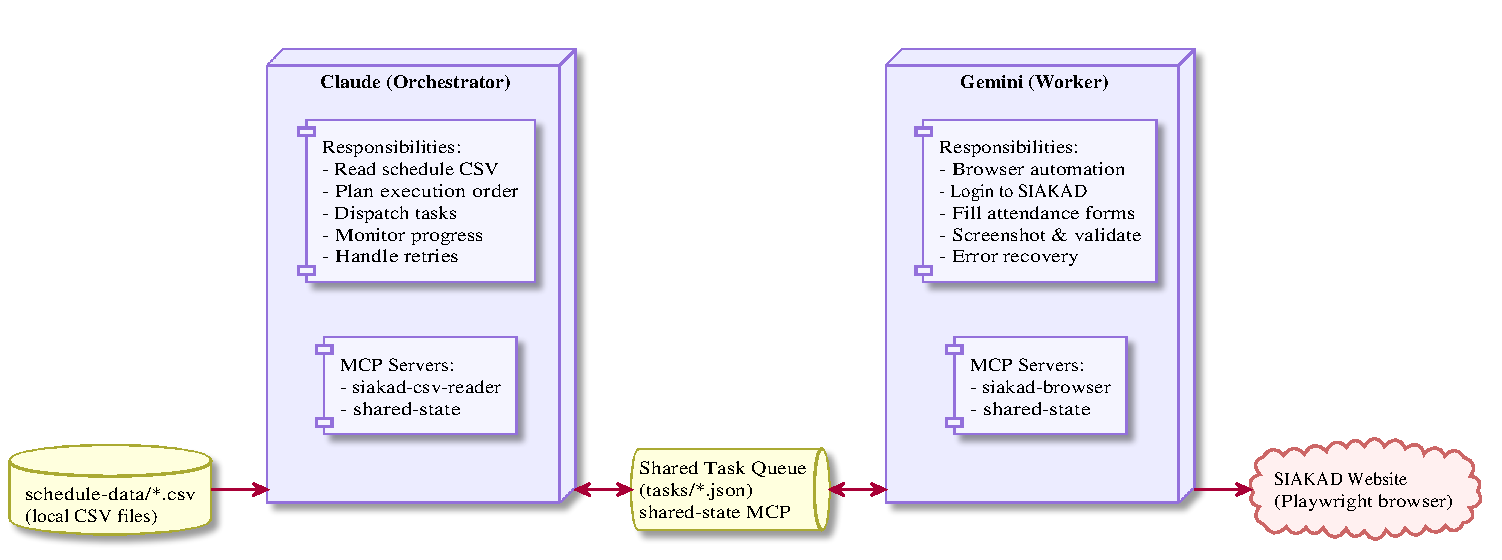
\includegraphics[width=1.06\textwidth]{../../figures/architecture.pdf}

\vspace{6pt}
\small
\textbf{4 komponen:} Data CSV $\rightarrow$ Claude (Orchestrator) $\leftrightarrow$ Shared Task Queue $\leftrightarrow$ Gemini (Worker) $\rightarrow$ SIAKAD Website
\end{frame}

\begin{frame}{Tiga Server MCP}
\vspace{6pt}
\centering
\footnotesize
\begin{tabular}{|l|l|l|p{5cm}|}
\hline
\rowcolor{blue!12}
\textbf{Server} & \textbf{Digunakan Oleh} & \textbf{Tools} & \textbf{Fungsi} \\
\hline
\texttt{siakad-csv-reader} & Claude & 4 tools & Membaca dan memfilter data jadwal CSV/Excel \\
\hline
\texttt{siakad-browser} & Gemini & 15 tools & Otomasi browser Playwright (login, navigasi, isi form, screenshot) \\
\hline
\texttt{shared-state} & Keduanya & 6 tools & Task queue berbasis berkas JSON di \texttt{tasks/} \\
\hline
\end{tabular}

\vspace{10pt}
\small
Setiap server diimplementasikan sebagai skrip Python yang dijalankan melalui \texttt{run.sh} dan berkomunikasi via transport \texttt{stdio}.
\end{frame}

\begin{frame}{Struktur Proyek}
\vspace{4pt}
\footnotesize
\begin{columns}[T]
\column{0.5\textwidth}
\textbf{Data Layer}
\begin{itemize}
  \item \texttt{config.json} --- kredensial, URL
  \item \texttt{schedule-data/*.csv} --- jadwal matkul
\end{itemize}

\vspace{6pt}
\textbf{Tool Layer (MCP Servers)}
\begin{itemize}
  \item \texttt{mcp-servers/csv-reader/}
  \item \texttt{mcp-servers/browser-automation/}
  \item \texttt{agents/shared\_state.py}
\end{itemize}

\column{0.5\textwidth}
\textbf{Agent Layer}
\begin{itemize}
  \item \texttt{agents/orchestrator\_prompt.md}
  \item \texttt{agents/worker\_prompt.md}
  \item \texttt{CLAUDE.md}, \texttt{GEMINI.md}
\end{itemize}

\vspace{6pt}
\textbf{Launch Scripts}
\begin{itemize}
  \item \texttt{run\_multiagents.sh} --- multi-agen
  \item \texttt{run\_claude\_only.sh} --- Claude saja
  \item \texttt{run\_gemini\_only.sh} --- Gemini saja
  \item \texttt{run\_claude\_interactive.sh} --- interaktif
\end{itemize}
\end{columns}
\end{frame}

% ============================================================
\section{Task Queue \& State Machine}
\begin{frame}{\hfill}
	\centering
	\Huge{\textbf{Task Queue \& State Machine}}
\end{frame}

\begin{frame}[fragile]{Format Tugas JSON}
\vspace{4pt}
\begin{columns}[T]
\column{0.5\textwidth}
\begin{lstlisting}[language=json, basicstyle=\ttfamily\tiny]
{
  "id": "task_002",
  "type": "fill_attendance",
  "status": "pending",
  "params": {
    "tanggal": "2026-01-21",
    "mata_kuliah": "Advanced Software
                    Engineering & DevOps",
    "kelompok_kelas": null,
    "semester": "2025/2026 GENAP",
    "topik": "Session-001: General Lecture",
    "deskripsi": "Overview of course objectives"
  },
  "result": null,
  "error": null,
  "created_at": "2026-04-04 10:30:15",
  "updated_at": null
}
\end{lstlisting}

\column{0.5\textwidth}
\vspace{10pt}
\textbf{State Machine Tugas}
\begin{center}
\scalebox{0.7}{
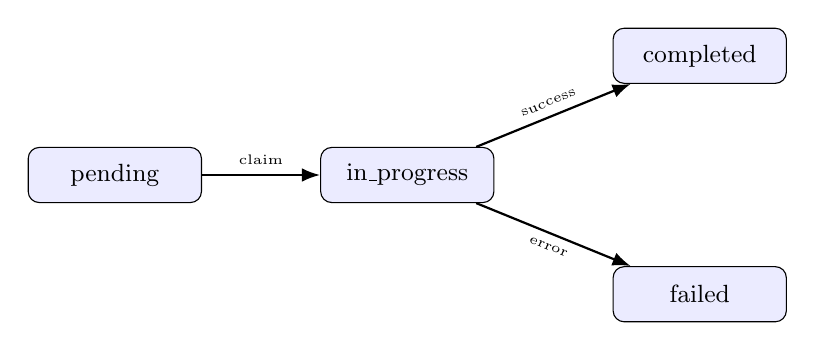
\begin{tikzpicture}[>=Latex, node distance=15mm,
  box/.style={draw,rounded corners,minimum width=2.2cm,minimum height=0.7cm,align=center,fill=blue!8,font=\small}]
  \node[box] (p) {pending};
  \node[box, right=of p] (ip) {in\_progress};
  \node[box, above right=8mm and 15mm of ip] (c) {completed};
  \node[box, below right=8mm and 15mm of ip] (f) {failed};
  \draw[->, thick] (p) -- node[above,font=\tiny]{claim} (ip);
  \draw[->, thick] (ip) -- node[above,font=\tiny,sloped]{success} (c);
  \draw[->, thick] (ip) -- node[below,font=\tiny,sloped]{error} (f);
\end{tikzpicture}
}
\end{center}

\vspace{6pt}
\textbf{Keunggulan}
\begin{itemize}
  \item Persisten: berkas JSON tetap ada.
  \item Inspectable: bisa dibuka manual.
  \item Mendukung retry.
\end{itemize}
\end{columns}
\end{frame}

% ============================================================
\section{Implementasi: CSV Reader}
\begin{frame}{\hfill}
	\centering
	\Huge{\textbf{Implementasi: CSV Reader}}
\end{frame}

\begin{frame}[fragile]{Server CSV Reader: Flexible Column Mapping}
\vspace{4pt}
\begin{columns}[T]
\column{0.45\textwidth}
\begin{lstlisting}[language=python, basicstyle=\ttfamily\tiny]
mcp = FastMCP("siakad-csv-reader")

@mcp.tool()
def read_attendance_data(file_path: str) -> str:
    df = pd.read_csv(file_path)
    # Flexible column mapping: tanggal/date, topik/topic, ...
    col_mapping = {}
    for col in df.columns:
        if "tanggal" in col or "date" in col:
            col_mapping["tanggal"] = col
        # ... similarly for mata_kuliah, topik, deskripsi

    # Normalize dates to YYYY-MM-DD
    df["tanggal"] = pd.to_datetime(
        df["tanggal"], dayfirst=True, format="mixed"
    ).dt.strftime("%Y-%m-%d")

    return json.dumps({"data": df.to_dict("records")})
\end{lstlisting}

\column{0.55\textwidth}
\vspace{10pt}
\textbf{4 Tools CSV Reader}
\begin{enumerate}
  \item \texttt{list\_schedule\_files(dir)}
  \item \texttt{read\_attendance\_data(path)}
  \item \texttt{get\_attendance\_for\_date(path, date)}
  \item \texttt{list\_attendance\_dates(path)}
\end{enumerate}

\vspace{8pt}
\textbf{Fitur kunci}
\begin{itemize}
  \item Mapping kolom fleksibel (tanggal $\leftrightarrow$ date, topik $\leftrightarrow$ topic).
  \item Konversi tanggal otomatis dari berbagai format.
  \item Support CSV dan Excel.
\end{itemize}
\end{columns}
\end{frame}

% ============================================================
\section{Implementasi: Browser Automation}
\begin{frame}{\hfill}
	\centering
	\Huge{\textbf{Implementasi: Browser Automation}}
\end{frame}

\begin{frame}[fragile]{Browser: Global State \& Lazy Init}
\vspace{4pt}
\begin{columns}[T]
\column{0.45\textwidth}
\begin{lstlisting}[language=python, basicstyle=\ttfamily\tiny]
mcp = FastMCP("siakad-browser")

# Global state - persists across tool calls
_playwright = None
_browser = None
_page = None

async def _ensure_browser():
    """Lazily initialize browser, return active page."""
    global _playwright, _browser, _page
    if _page is None or _page.is_closed():
        _playwright = await async_playwright().start()
        _browser = await _playwright.chromium.launch(
            headless=False, slow_mo=100)
        ctx = await _browser.new_context(
            viewport={"width": 1248, "height": 900})
        _page = await ctx.new_page()
    return _page
\end{lstlisting}

\column{0.55\textwidth}
\vspace{10pt}
\textbf{Pola Desain}
\begin{itemize}
  \item \textbf{Lazy init:} Browser hanya dibuat saat tool pertama dipanggil.
  \item \textbf{Global state:} Satu sesi browser bertahan sepanjang lifecycle server.
  \item \textbf{Visible mode:} \texttt{headless=False} agar pengguna bisa memantau.
  \item \textbf{Slow motion:} 100ms jeda antar-aksi untuk stabilitas.
  \item \textbf{Adaptive viewport:} 65\% lebar monitor.
\end{itemize}
\end{columns}
\end{frame}

\begin{frame}[fragile]{Browser: Login dengan Multi-Selector}
\vspace{4pt}
\begin{columns}[T]
\column{0.45\textwidth}
\begin{lstlisting}[language=python, basicstyle=\ttfamily\tiny]
@mcp.tool()
async def login_siakad(username="", password=""):
    page = await _ensure_browser()
    try:
        await page.goto(SIAKAD_LOGIN_URL, wait_until="networkidle")
        # Multi-selector: works even if HTML structure changes
        await page.fill('input[name="username"], #username', username)
        await page.fill('input[name="password"], #password', password)
        await page.click('button[type="submit"], .btn-login')
        return f"Login OK. Title: {await page.title()}"
    except Exception as e:
        await page.screenshot(path="/tmp/login_error.png")
        return f"Error: {str(e)}"
\end{lstlisting}

\column{0.55\textwidth}
\vspace{10pt}
\textbf{Pola: Multi-Selector}
\begin{itemize}
  \item Beberapa CSS selector dipisahkan koma.
  \item Tool tetap berfungsi meskipun HTML berubah.
  \item Contoh: \texttt{input[name="username"]} atau \texttt{\#username} atau \texttt{input[type="email"]}.
\end{itemize}

\vspace{6pt}
\textbf{Pola: Error Screenshot}
\begin{itemize}
  \item Screenshot otomatis saat terjadi exception.
  \item Agen LLM dapat menggunakan gambar ini untuk mendiagnosis masalah.
\end{itemize}
\end{columns}
\end{frame}

\begin{frame}[fragile]{Browser: Date Picker --- 3 Strategi}
\vspace{4pt}
\begin{columns}[T]
\column{0.45\textwidth}
\begin{lstlisting}[language=python, basicstyle=\ttfamily\tiny]
@mcp.tool()
async def set_date_picker(date_str: str) -> str:
    page = await _ensure_browser()
    # Strategy 1: CSS selector
    el = await page.query_selector('input[type="date"], input.datepicker')
    if el:
        await el.fill(date_str)
        await el.dispatch_event("change")
        return "Date set"
    # Strategy 2: Placeholder-based
    els = await page.query_selector_all('input[placeholder*="tanggal"]')
    if els:
        await els[0].fill(us_date); return "Date set via placeholder"
    # Strategy 3: JavaScript fallback
    await page.evaluate("""(d) => {
        document.querySelectorAll('input').forEach(el => {
            if (el.type==='date') { el.value = d;
              el.dispatchEvent(new Event('change')); }
        });
    }""", date_str)
    return "Date set via JS"
\end{lstlisting}

\column{0.55\textwidth}
\vspace{10pt}
\textbf{Progressive Fallback}
\begin{enumerate}
  \item \textbf{Strategi 1:} Selector CSS spesifik (\texttt{input[type=date]}).
  \item \textbf{Strategi 2:} Deteksi via placeholder text.
  \item \textbf{Strategi 3:} JavaScript langsung --- last resort.
\end{enumerate}

\vspace{8pt}
\textbf{Event dispatch} \texttt{change} memicu AJAX reload tabel jadwal setelah tanggal berubah.

\vspace{8pt}
\textbf{Format tanggal}\\
Tool menghitung tiga format sekaligus: \texttt{YYYY-MM-DD}, \texttt{MM/DD/YYYY}, \texttt{DD/MM/YYYY}.
\end{columns}
\end{frame}

\begin{frame}{15 Tools Browser Automation}
\vspace{20pt}
\centering
\scriptsize
\begin{tabular}{|c|l|p{7.5cm}|}
\hline
\rowcolor{blue!12}
\textbf{No} & \textbf{Tool} & \textbf{Fungsi} \\
\hline
1 & \texttt{launch\_browser} & Meluncurkan instance Chromium \\
\hline
2 & \texttt{login\_siakad} & Login ke portal SIAKAD \\
\hline
3 & \texttt{navigate\_to\_daftar\_hadir} & Navigasi ke halaman daftar hadir \\
\hline
4 & \texttt{set\_semester} & Memilih semester pada dropdown \\
\hline
5 & \texttt{set\_date\_picker} & Menetapkan tanggal (3 strategi fallback) \\
\hline
6 & \texttt{click\_search\_or\_filter} & Mengklik tombol cari/filter \\
\hline
7 & \texttt{get\_schedule\_list} & Mengambil data tabel jadwal sebagai JSON \\
\hline
8 & \texttt{find\_schedule\_row} & Mencari baris berdasarkan mata kuliah \& kelas \\
\hline
9 & \texttt{click\_absensi\_button} & Mengklik tombol Absensi pada baris tertentu \\
\hline
10 & \texttt{fill\_attendance\_form} & Mengisi topik dan deskripsi pada popup modal \\
\hline
11 & \texttt{submit\_attendance\_form} & Menyimpan formulir kehadiran \\
\hline
12 & \texttt{take\_screenshot} & Mengambil tangkapan layar (debugging) \\
\hline
13 & \texttt{get\_page\_html} & Mengambil konten HTML halaman \\
\hline
14 & \texttt{run\_js} & Menjalankan JavaScript arbitrary \\
\hline
15 & \texttt{close\_browser} & Menutup browser dan cleanup resources \\
\hline
\end{tabular}

\vspace{4pt}
\small
Tools 12--14 berfungsi sebagai \textit{debugging escape hatch} bagi agen.
\end{frame}

% ============================================================
\section{Implementasi: Shared State}
\begin{frame}{\hfill}
	\centering
	\Huge{\textbf{Implementasi: Shared State}}
\end{frame}

\begin{frame}[fragile]{Shared State: Task Queue}
\vspace{4pt}
\begin{columns}[T]
\column{0.55\textwidth}
\begin{lstlisting}[language=python, basicstyle=\ttfamily\tiny]
mcp = FastMCP("shared-state")
TASKS_DIR = Path(__file__).parent.parent / "tasks"

@mcp.tool()
def create_task(task_id, task_type, params):
    task = {"id": task_id, "type": task_type,
            "status": "pending", "params": json.loads(params)}
    (TASKS_DIR / f"{task_id}.json").write_text(json.dumps(task))
    return f"Task '{task_id}' created."

@mcp.tool()
def update_task(task_id, status, result="", error=""):
    path = TASKS_DIR / f"{task_id}.json"
    task = json.loads(path.read_text())
    task["status"] = status
    if result: task["result"] = result
    if error:  task["error"] = error
    path.write_text(json.dumps(task))
    return f"Task '{task_id}' -> '{status}'."
\end{lstlisting}

\column{0.45\textwidth}
\vspace{10pt}
\textbf{6 Tools Shared State}
\begin{itemize}
  \item \texttt{create\_task}, \texttt{get\_task}, \texttt{update\_task}, \texttt{list\_tasks}, \texttt{get\_next\_pending\_task}, \texttt{clear\_tasks}
\end{itemize}

\vspace{6pt}
\textbf{Desain}
\begin{itemize}
  \item Setiap tugas = 1 berkas JSON, Tidak perlu database, Persisten terhadap restart.
  \item \textbf{Orchestrator}: create \& get, \textbf{Worker}: get\_next \& update.
\end{itemize}
\end{columns}
\end{frame}

% ============================================================
\section{Agent Prompt \& Alur Kerja}
\begin{frame}{\hfill}
	\centering
	\Huge{\textbf{Agent Prompt \& Alur Kerja}}
\end{frame}

\begin{frame}{Orchestrator vs Worker: Pembagian Tugas}
\vspace{4pt}
\centering
\scriptsize
\begin{tabular}{|>{\raggedright\arraybackslash}p{0.14\textwidth}|>{\raggedright\arraybackslash}p{0.37\textwidth}|>{\raggedright\arraybackslash}p{0.37\textwidth}|}
\hline
\rowcolor{blue!12}
\textbf{Aspek} & \textbf{Orchestrator (Claude)} & \textbf{Worker (Gemini)} \\
\hline
Peran & Perencana dan pengirim tugas & Pelaksana otomasi browser \\
\hline
Server MCP & \texttt{csv-reader}, \texttt{shared-state} & \texttt{browser}, \texttt{shared-state} \\
\hline
Fokus & Membaca data, validasi, dispatch & Login, navigasi, isi form, screenshot \\
\hline
Interaksi & Tidak berinteraksi dengan browser & Tidak membaca data jadwal \\
\hline
Error handling & Retry dengan task ID baru & Screenshot + fallback selector \\
\hline
\end{tabular}

\vspace{8pt}
\small
\textbf{Prinsip kunci:} Setiap agen hanya menerima konteks yang relevan --- \textit{separation of concerns} mengurangi konsumsi token dan meningkatkan akurasi.
\end{frame}

\begin{frame}{Alur Kerja Orchestrator (8 Langkah)}
\vspace{6pt}
\begin{columns}[T]
\column{0.5\textwidth}
\begin{enumerate}
  \item \texttt{clear\_tasks()} --- bersihkan antrean.
  \item \texttt{list\_schedule\_files()} --- temukan CSV.
  \item \texttt{read\_attendance\_data()} --- baca data.
  \item \texttt{create\_task("login")} --- dispatch login.
\end{enumerate}

\column{0.5\textwidth}
\begin{enumerate}
  \setcounter{enumi}{4}
  \item Poll \texttt{get\_task()} --- tunggu login selesai.
  \item Loop: \texttt{create\_task("fill\_attendance")} per record. Tunggu selesai sebelum dispatch berikutnya.
  \item \texttt{create\_task("close\_browser")}.
  \item Print summary --- laporan akhir.
\end{enumerate}
\end{columns}

\vspace{8pt}
\small
\textbf{Aturan penting:} Satu tugas pada satu waktu --- Orchestrator selalu menunggu tugas sebelumnya selesai sebelum mengirim tugas baru.
\end{frame}

\begin{frame}{Aturan Keandalan Worker}
\vspace{6pt}
\begin{enumerate}
  \item \textbf{One Step at a Time.} Jangan chain multiple browser tools dalam satu turn --- tunggu hasil setiap langkah.
  \item \textbf{Handle Loader.} Setelah set tanggal/semester, tunggu \texttt{div.box\_loader} menghilang (halaman refresh via AJAX).
  \item \textbf{Overwrite Policy.} Selalu REPLACE topik dan deskripsi yang sudah ada --- \texttt{fill()} otomatis menghapus teks lama.
  \item \textbf{Saving Fallback.} Jika \texttt{submit\_attendance\_form} gagal, panggil \texttt{save\_pembahasan()} via \texttt{run\_js}.
  \item \textbf{Verify Success.} Cek pesan ``Sukses update topik pembahasan'' setelah save menggunakan \texttt{get\_page\_html} atau \texttt{run\_js}.
\end{enumerate}
\end{frame}

\begingroup
\setbeamercolor{background canvas}{bg=white}
\begin{frame}{}
    \begin{columns}[c] % 'c' vertically centers the content in both columns
        
        % Left Column: Text
        \begin{column}{0.35\textwidth}
            \centering
			\vspace{2pt}
            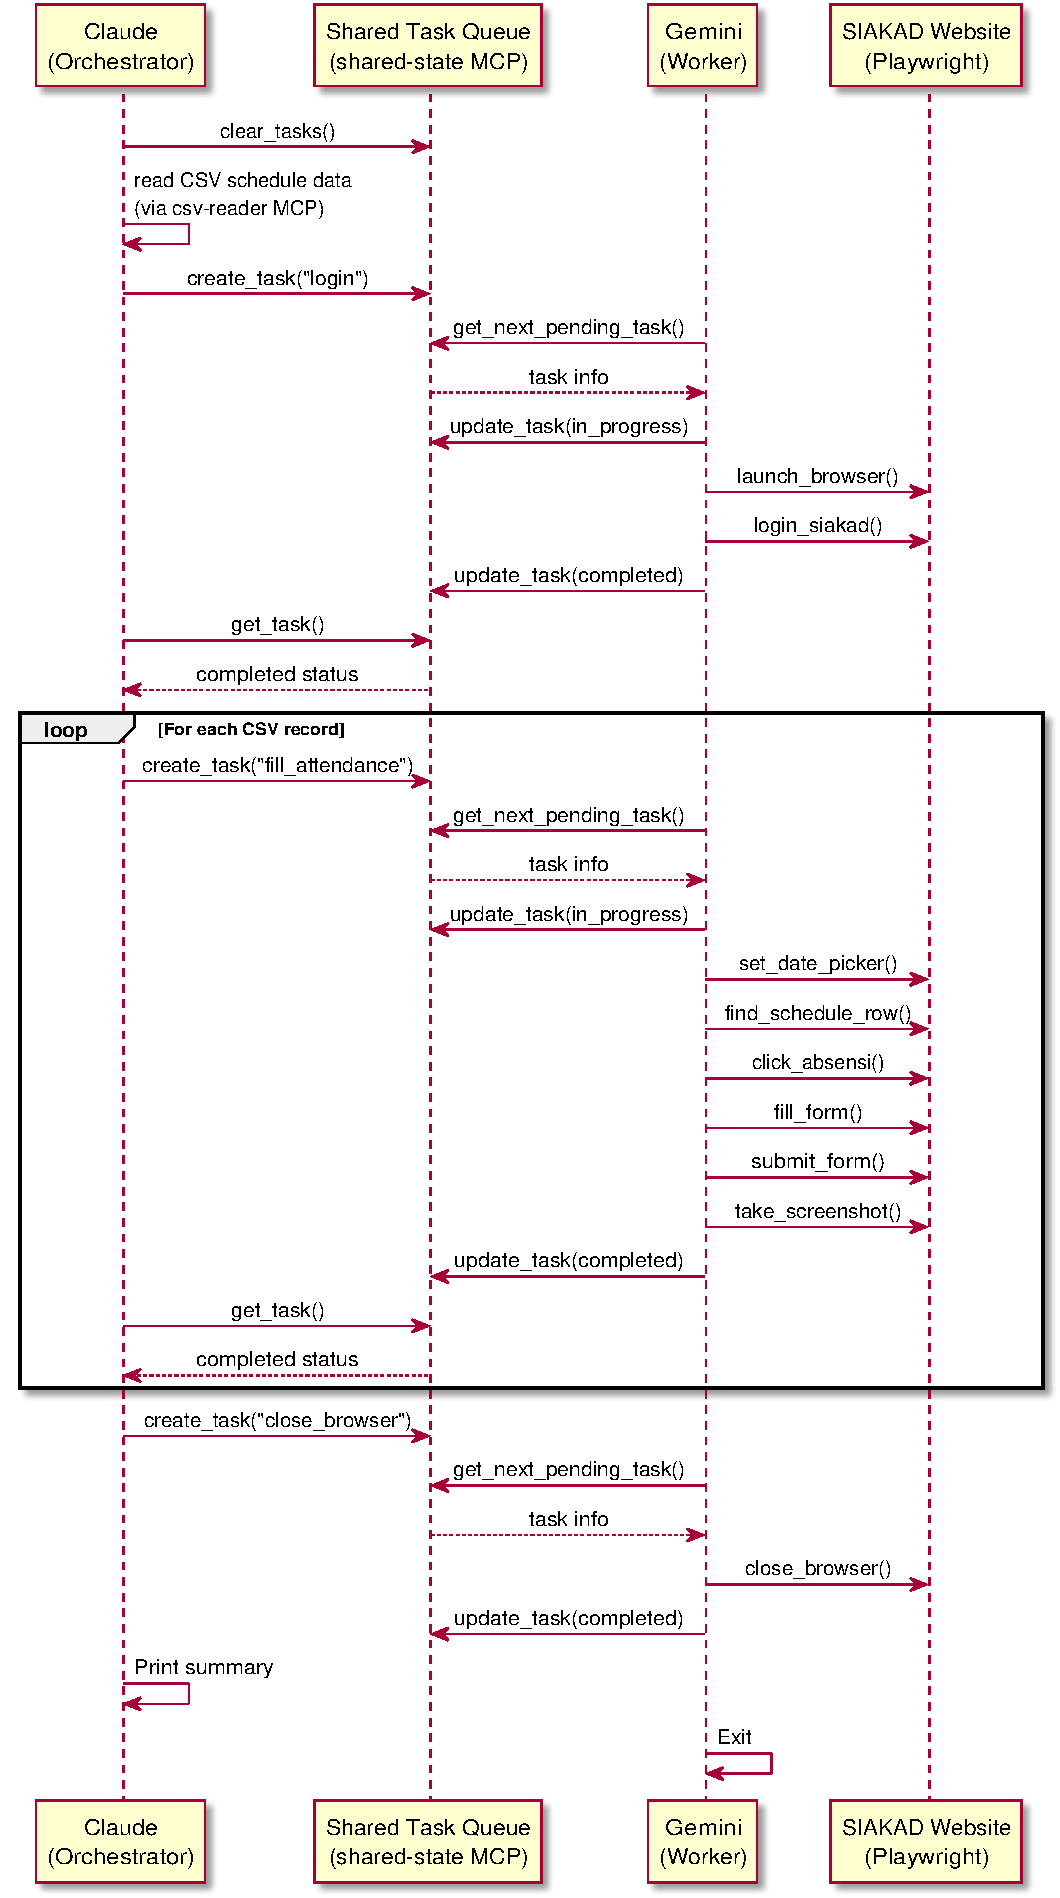
\includegraphics[width=\textwidth]{../../figures/sequence.pdf}
        \end{column}
        
        % Right Column: Figure
        \begin{column}{0.5\textwidth}
			\textbf{Diagram Sekuens Interaksi}
			\vspace{10pt}

            \textbf{Lima fase:} Inisialisasi $\rightarrow$ Login $\rightarrow$ Pengisian (Loop) $\rightarrow$ Penutupan $\rightarrow$ Laporan.
        \end{column}
        
    \end{columns}
\end{frame}
\endgroup

\begin{frame}[fragile]{Skrip Peluncuran Multi-Agen}
\vspace{4pt}
\begin{lstlisting}[language=bash, basicstyle=\ttfamily\tiny]
#!/bin/bash
rm -f "$SCRIPT_DIR/tasks/"*.json  # Clean previous tasks

# Register Gemini MCP servers
gemini mcp add --scope project siakad-browser \
  "$SCRIPT_DIR/mcp-servers/browser-automation/run.sh" -e DISPLAY=:0
gemini mcp add --scope project shared-state \
  "$SCRIPT_DIR/agents/run_shared_state.sh"

# Step 1: Start Gemini (Worker) in background
gemini --yolo --model gemini-3-flash-preview --prompt "
  $WORKER_PROMPT
  Poll get_next_pending_task until close_browser task.
" &
GEMINI_PID=$!; sleep 3

# Step 2: Start Claude (Orchestrator) in foreground
claude -p --mcp-config "$MCP_CONFIG_FILE" --dangerously-skip-permissions <<PROMPT
  $ORCHESTRATOR_PROMPT
  Schedule directory: $SCHEDULE_DIR
  Execute the workflow. Start now.
PROMPT

wait $GEMINI_PID  # Wait for Worker to finish
\end{lstlisting}
\end{frame}

% ============================================================
\section{Perbandingan \& Evaluasi}
\begin{frame}{\hfill}
	\centering
	\Huge{\textbf{Perbandingan \& Evaluasi}}
\end{frame}

\begin{frame}{Multi-Agent vs Single-Agent}
\vspace{4pt}
\centering
\footnotesize
\begin{tabular}{|>{\raggedright\arraybackslash}p{0.14\textwidth}|>{\raggedright\arraybackslash}p{0.37\textwidth}|>{\raggedright\arraybackslash}p{0.37\textwidth}|}
\hline
\rowcolor{blue!12}
\textbf{Aspek} & \textbf{Multi-Agent (Claude + Gemini)} & \textbf{Single-Agent} \\
\hline
Keandalan & Tinggi; task queue persisten, mendukung retry. & Sedang; kegagalan sering ulang dari awal. \\
\hline
Efisiensi Token & Sangat baik; tiap agen menerima konteks relevan saja. & Kurang; seluruh data + riwayat browser sekaligus. \\
\hline
Visual Reasoning & Kuat; Gemini dioptimalkan untuk visual web. & Terbatas (Claude saja); kuat (Gemini saja). \\
\hline
Skalabilitas & Dapat paralel beberapa Worker. & Satu alur sekuensial. \\
\hline
Kompleksitas & Lebih tinggi; perlu task queue + skrip launch. & Lebih rendah; satu skrip + satu prompt. \\
\hline
Debugging & Mudah; JSON inspectable + screenshot per langkah. & Sulit; konteks di satu log agen. \\
\hline
\end{tabular}
\end{frame}

\begin{frame}{4 Mode Eksekusi}
\vspace{6pt}
\centering
\footnotesize
\begin{tabular}{|l|l|p{6.5cm}|}
\hline
\rowcolor{blue!12}
\textbf{Skrip} & \textbf{Agen} & \textbf{Keterangan} \\
\hline
\texttt{run\_multiagents.sh} & Claude + Gemini & Mode utama; paling andal. \\
\hline
\texttt{run\_claude\_only.sh} & Claude saja & Lebih sederhana, kurang visual reasoning. \\
\hline
\texttt{run\_gemini\_only.sh} & Gemini saja & Cocok untuk pengujian cepat. \\
\hline
\texttt{run\_claude\_interactive.sh} & Claude (chat) & Untuk debugging step-by-step. \\
\hline
\end{tabular}

\vspace{10pt}
\small
\textbf{Pilih Multi-Agent} jika data banyak ($>$5 sesi) dan keandalan prioritas.\\
\textbf{Pilih Single-Agent} jika data sedikit atau hanya satu CLI tersedia.\\
\textbf{Pilih Interactive} untuk debugging atau pengisian manual terbimbing.
\end{frame}

% ============================================================
\section{Risiko \& Mitigasi}
\begin{frame}{\hfill}
	\centering
	\Huge{\textbf{Risiko \& Mitigasi}}
\end{frame}

\begin{frame}{Risiko dan Pitfall Umum}
\vspace{6pt}
\footnotesize
\begin{enumerate}
  \item \textbf{Race condition task queue.} JSON tanpa locking $\rightarrow$ dispatch satu per satu, Orchestrator hanya write, Worker hanya update.
  \item \textbf{Perubahan HTML SIAKAD.} Selector bisa usang $\rightarrow$ multi-selector fallback + debugging tools (\texttt{get\_page\_html}, \texttt{run\_js}).
  \item \textbf{Timeout halaman loading.} AJAX reload lambat $\rightarrow$ Worker wajib cek \texttt{div.box\_loader} setelah set tanggal/semester.
  \item \textbf{Tugas stuck \texttt{in\_progress}.} Worker crash sebelum report $\rightarrow$ prompt rule: ``never leave task in in\_progress''; \texttt{clear\_tasks} saat restart.
  \item \textbf{Format tanggal inkonsisten.} Locale berbeda $\rightarrow$ tool menghitung 3 format (YYYY-MM-DD, MM/DD/YYYY, DD/MM/YYYY) dan coba secara progresif.
  \item \textbf{Sinkronisasi startup.} Orchestrator mulai sebelum Worker siap $\rightarrow$ \texttt{sleep 3} + dispatch sekuensial.
\end{enumerate}
\end{frame}

% ============================================================
\section{Ringkasan}
\begin{frame}{\hfill}
	\centering
	\Huge{\textbf{Ringkasan}}
\end{frame}

\begin{frame}{Kesimpulan Sesi}
\vspace{15pt}
\begin{itemize}
  \item Multi-Agent System berbasis MCP efektif untuk otomasi proses bisnis yang melibatkan antarmuka web dinamis dan data input besar.
  \item Pemisahan peran: \textbf{Claude} (Orchestrator) menangani planning \& task management; \textbf{Gemini} (Worker) menangani browser automation \& visual reasoning.
  \item \textbf{3 server MCP modular:} \texttt{csv-reader} (4 tools), \texttt{browser} (15 tools), \texttt{shared-state} (6 tools) --- total 25 tools.
  \item \textbf{Task queue} berbasis berkas JSON: sederhana, persisten, inspectable, mendukung retry.
  \item \textbf{Agent prompt engineering} mengatur perilaku agen melalui instruksi terstruktur: workflow, reliability rules, error handling.
  \item Trade-off: kompleksitas infrastruktur meningkat, tetapi keandalan, efisiensi konteks, dan kemampuan debugging jauh lebih baik.
\end{itemize}
\end{frame}

\end{document}
